\chapter{Introduction}

\section{Internet des Objets}

\subsection{Définition}
Le terme Internet des Objets décrit le réseau d'appareils physiques - souvent hétérogène - interconnectés, et dont le rôle principal est la récolte et l'échange d'information, ainsi que l'interaction avec l'environnement extérieur \cite{patel2016}. Cette infrastructure est dite intelligente, dotée de la capacité de s'auto-organiser, partager l'information de manière optimale et de réagir aux changements environnementaux \cite{madakam2015}.\par
Les objets dans ce type de réseau sont de capacité limitée, que ce soit en puissance de calcul ou en consommation d'énergie. Ce sont majoritairement des objets électroniques quotidiens (à l'exemple de smartphones, véhicules ou équipements ménagers), chacun avec sa propre identité, pour communiquer avec le reste des objets, et synchroniser les efforts de réponses aux différentes situations externes auxquelles ils sont exposés.

\subsection{Histoire et Évolution}
L'idée d'interconnecter des dispositifs électroniques moyennant un réseau informatique est apparue dans les années 80s, à l'Université de Carnegie Melon, où on avait relié un distributeur de boissons fraîches à un ordinateur de monitorage. Ce qui a permis aux programmeurs de consulter la disponibilité des boissons à distance et d'éviter les trajets inutiles \cite{madakam2015}.\par
Cependant, le premier à avoir introduit ce concept est Kevin Ashton en 1999, qui travaillait dans l'optimisation de chaîne de production chez Procter \& Gamble. Dans sa présentation portant le nom de la technologie, il a développé l'idée de décharger l'homme de la tâche de récolte d'information (en 1999, 50 petabytes d'information était créée par des êtres humains), et de plutôt exploiter la masse d'engins et capteurs disponibles déjà déployés à ce moment là \cite{ashton2009}.\par
Cette infrastructure n'a été adoptée en industrie qu'en fin années 2000s, où le ratio d'objets/hommes est passé à 1.84 pour 0.08 en 2003. Depuis, les constructeurs du domaine de téléinformatique concentrent leurs efforts sur la production de capteurs et d'appareils IoT avec différentes fonctionnalités dans le but de combler les besoins des diverses industries, allant de l'agriculture et domaine médical, jusqu'à l'industrie militaire

\subsection{Architecture}
L'architecture d'un réseau Iot se décompose en 4 couches flexibles. Chaque couche est constituée de plusieurs technologies et standards \cite{patel2016}. Cet aspect modulaire permet une meilleure scalabilité de l'infrastructure et une meilleure adaptation aux besoins émergeants. Les couches de ce modèle sont comme suit:
\begin{enumerate}
  \item \emph{La couche de capteurs et d'objets intelligents:} Elle est formée d'objets connectés munis de capteurs et/ou d'actionneurs. C'est la couche la plus proche de l'environnement physique, celle-ci transforme les événements générés par ce dernier en un flux d'information à temps réel, et se charge de leur transmission. Les capteurs ont différentes spécifications, comme la mesure de la température, pression, capture de mouvement …, et sont soit connectés à des passerelles à l'aide de réseaux filaires (Ethernet) ou non (Wi-Fi, Bluetooth, RFID …), soit directement à la couche applicative. Un exemple de ce type de technologie sont les WSNs, caractérisés par leur basse consommation d'énergie et grande zone de couverture.
  \item \emph{La couche réseau et passerelles:} Cette couche garantit la transmission de la masse d'information générée par la couche précédente, tout en respectant la qualité de service exigée par les applications servies. Plusieurs infrastructures et protocoles de communication ont été mis en place dans le but d'optimiser l'acheminement et traitement d'information, comme le concept de Fog Computing qu'on détaillera par la suite.
  \item \emph{La couche de gestion:} Le rôle de cette couche est de filtrer et organiser les informations, en fournissant une couche d'abstraction à l'application. Elle s'occupe de la gestion de priorité, et l'analyse de la pertinence des données. C'est aussi à ce niveau que les politiques d'anonymisation et sécurisation de données sont implémentées.
  \item \emph{La couche d'application:} Elle est située majoritairement dans des clouds ou data-centers. Les applications couvrent des domaines différents comme l'agriculture et la gestion de villes intelligentes, et d'autres plus critiques comme le domaine de la santé ou le domaine militaire. Toutefois, depuis quelques années, les efforts de recherches visent à rapprocher ces applications de la première couche du modèle.
\end{enumerate}

\subsection{Quelque domaines d'application}
L'installation d'objets intelligents s'est démocratisée depuis quelques années. On les retrouve dans les environnements suivants:
\begin{itemize}
  \item Les systèmes de sécurité et surveillance, où des caméras et capteurs de mouvements permettent de détecter et identifier toute activité suspecte.
  \item Les maisons intelligentes: ce qui décrit la connectivité des objets dans un domicile, tous œuvrent pour fournir de meilleures conditions de vie, et ceci en assurant: la régulation de températures, l'optimisation de consommation d'énergie, la détection d'incendie et le filtrage de l'air.
  \item Les systèmes de voitures autonomes dans lesquels les véhicules utilisant la voie publique peuvent s'échanger des informations, parfois critiques, et alerter les conducteurs de tout danger imminent. Ils peuvent aussi, en se basant sur les informations de géolocalisation fournies par les autres usagers, produire des recommandations de destination tout en évitant les points de congestion de la circulation routière.
  \item Les dispositifs permettant la surveillance médicale de personnes incapacités, et ainsi prise de dispositions nécessaires dans les moments d'urgence.
\end{itemize}

\subsection{Problèmes et difficultés}
Avec la croissance du nombre d'objets connectés, les attaques cybercriminelles deviennent excentriques. Ce réseau peut être vulnérable contre l'injection de données erronées qui peuvent influencer des prises de décision parfois critiques. Les nœuds intercommunicants disposent de ressources limitées, et ainsi, ils peuvent être sujets à des attaques de déni de service DDOS. La grande quantité de données produite doit être protégée tout au long du circuit liant les couches présentées précédemment. Un travail de supervision doit être mené dans le but de garantir la confidentialité des données récoltées, et empêcher les pratiques abusives comme la vente de données d'utilisateurs.\par
Le provisionnement en énergie est devenu une des préoccupations de la société actuelle. On cherche à optimiser l'utilisation de ressources énergétiques, soit pour étendre l'autonomie des objets et capteurs mobiles, ou bien pour réduire les frais d'approvisionnement en électricité. Des algorithmes de gestion et allocation des ressources ont été proposés pour minimiser cette consommation, mais les recherches sur ce sujet sont toujours actives.\par
De plus, certaines applications demandent une certaine réactivité et une grande vitesse de réponse pour accomplir des missions critiques comme pour la conduite de véhicules automobiles ou la surveillance médicale. Ces exigences sont souvent restreintes par d'autres contraintes comme la mobilité des objets connectés ou la congestion dans le réseau de communication.
%------------------------------------------------------------
\section{Fog Computing}

\subsection{Histoire et évolution}
Malgré les avantages considérables que procure le \emph{Cloud computing} en termes de performance, d'accessibilité et de scalabilité, il trouve néanmoins quelques limites face à l'expansion de l'internet des objets (IoT), ce qui impose donc une réévaluation de ce paradigme. \par 
En effet, l'accélération de la croissance du nombre d'appareils connectés à internet ainsi que l'énorme quantité de données générées par ces derniers ont démontré une certaine limitation du paradigme \emph{Cloud}. Le problème le plus apparent est le problème de latence, en vue donc de la croissance de la quantité de données générée par les différents objets connectés et la dépendance de ces derniers visé à vis du \emph{Cloud} pour le traitement de ces données, ceci risque de provoquer une réduction considérable des performances du réseau, ce qui engendrerait une augmentation des délais de transfert et donc une diminution des performances de traitement. Ce qui peut être critique au niveau de certaines applications notamment les applications qui requièrent des traitements en temps réel.\\
D'autres problèmes peuvent être cités également, comme le problème de congestion ou encore le problème de connaissance de localisation. \par
C'est pour répondre donc à ces problèmes que le \emph{Fog computing} a été proposée comme une extension du paradigme \emph{Cloud} en 2012, et qui a vu par la suite la création d'un consortium dédié qu'est l'\textbf{OpenFog Consortium} afin de faciliter l'interopérabilité des différentes solutions technologiques.
\subsection{Définition et concept}
Selon la définition proposée par CISCO \cite{bonomi2012}, le terme \emph{Fog computing} désigne : \og{}une plate-forme hautement virtualisée qui fournit des services de calcul, de stockage et de mise en réseau entre les appareils finaux et les centres de données de \emph{Cloud computing} traditionnels, généralement, mais pas exclusivement, située à la périphérie du réseau\fg{}.\par
L'OpenFog Consortium \cite{OpenFog2017} le définit aussi comme étant : \og{} Une architecture horizontale au niveau du système qui distribue des fonctions de calcul, de stockage, de contrôle et de mise en réseau plus proches des utilisateurs le long du continuum \emph{Cloud-objet}\fg{}.\par
Le terme réfère aussi à une infrastructure matérielle et applicative distribuée qui vise à stocker et à traiter les données issues des différents appareils connectés afin de se substituer au \emph{Cloud} pour certains traitements.\par
La principale idée du \emph{Fog computing} est l'instrumentalisation des différents équipements qui constitue les noeuds du réseau (routeurs, commutateurs, passerelles, etc.) comme étant un centre de traitement et de stockage de donnés distribué qui est à la fois intermédiaire au \emph{Cloud} et en même temps proche des extrémités du réseau.
En créant donc une couche auprès de la production des données, ceci entraîne une réduction des transferts entrant et sortant du \emph{Cloud} et donc une réduction de la latence, et par conséquent le temps des différents traitements et services.
\subsection{Architecture}
La plupart des recherche qui s'oriente vers la définition d'un modèle architectural semblent se diriger vers un même modèle, à savoir un modèle en 3 couches\cite{de2019}.\\
Les couches de ce modèle sont présenté comme suit :
\begin{itemize}
  \item \emph{Couche IoT:} Cette couche désigne l'ensemble des appareils se trouvant à l'extrémité du réseau, elle est composée essentiellement d'appareils IoT tels que des véhicules intelligents, des smartphones, des drones militaires, des capteurs sensoriels, etc. Le rôle de ces derniers étant la collecte et la transmission des données vers la couche supérieure pour stockage ou traitement.
  \item \emph{Couche de Fog:} Cette couche constitue le point central du paradigme \emph{Fog}, elle est constituée d'un ensemble de nœuds \emph{Fog}, qui selon le OpenFog Consortium, ce dernier se définit comme 
  \og{}un élément physique ou logique qui implémente les services informatiques \emph{Fog}\fg\cite{de2019}.\par
  L'ensemble des nœuds constitue un centre de traitement et de stockage distribué connecté à la fois à la couche inférieure et celle supérieure à travers des nœuds passerelles. Permettant ainsi de bénéficier des différents services fournis par la couche supérieure qu'est le \emph{Cloud} par exemple le stockage, tout en fournissant des informations contextuelles aux utilisateurs au niveau de la couche inférieure.
  \item \emph{Couche cloud:} Cette couche représente une infrastructure \emph{Cloud} centralisée , elle composé de ressource matérielle élevé et fournit différent service, ayant comme différences avec une architecture en \emph{Cloud} classique, certains traitements et services sont déchargés de la couche \emph{Cloud} au profit de la couche \emph{Fog} afin d'équilibrer la charge de travail et d'augmenter l'efficacité et la fiabilité.
\end{itemize}
\subsection{Avantages}
Le Fog computing présente de nombreux avantages qui convient de souligner, ils sont généralement résumés sous le sigle SCALE pour :
\begin{itemize}
  \item \emph{Sécurité:} Dans ce paradigme, la sécurité est prise en considération lors de l'élaboration de l'architecture plutôt qu'une partie optionnelle.
  \item \emph{Cognition:} Vient du fait que l'infrastructure \emph{Fog} est consciente des besoins et exigences des utilisateurs, ainsi elle distribue plus finement les ressources en fonction de chaque utilisateur contrairement au \emph{Cloud}.
  \item \emph{Agilité:} Ce qui désigne la capacité d'adaptation rapide à l'innovation.
  \item \emph{Latence:} En raison de sa proximité avec les utilisateurs finaux, le \emph{Fog} a la capacité de supporter des applications qui nécessitent des latences courtes et stables, évitant ainsi les problèmes résultant des systèmes centralisés.
  \item \emph{Efficacité:} Vient du fait que cette vision étant les capacités du \emph{Cloud} en intégrant
  les différents nœuds qui composent le réseau à l'infrastructure de traitement et de stockage, augmentant ainsi la capacité ainsi que l'efficacité globale du système.
\end{itemize}
\subsection{Défis et verrous scientifiques}
Bien que le \emph{Fog computing} ait apporté des avantages considérable, ce paradigme reste relativement récent et nécessite  d'investiguer certains défis, par exemple :
\begin{itemize}
  \item \emph{Gestion de l'énergie:} Les infrastructures de \emph{Fog} comprennent généralement un grand nombre de nœuds géo-distribués. La consommation énergétique est donc plus élevée en comparaison avec celle du \emph{Cloud}. De grands efforts de recherches sont alors nécessaires pour développer des solutions efficaces afin de minimiser l'empreinte énergétique, par exemple, des algorithmes de traitement et des protocoles de communication moins coûteux en énergie sont à développer.
  \item \emph{Hétérogénéité:} En plus de l'hétérogénéité trouvé dans les environnement \emph{iot}, au nivaux des types d'objet connecté,des données, des technologies de communications et des performances. Ce problème est également présent dans les infrastructures \emph{Fog} en raison de la diversité des équipements qui constituent les nœuds \emph{Fog}. La gestion de l'hétérogénéité dans un environnement de \emph{Fog} et d'IoT représente  un défi important.
  \item \emph{Gestion et provision de ressources:} Les noeuds \emph{Fog} sont généralement des équipement à capacité limitée, il par conséquent indispensable de disposer de solution efficaces en termes de gestion de ressource, comme par exemple l'ordonnancement des différentes applications.
\end{itemize}
%------------------------------------------------------------
\section{Migration de Conteneurs}
\subsection{Définitions et concepts}
La virtualisation introduit une couche d'abstraction logicielle entre le matériel et le système d'exploitation ou les applications qui s'exécutent dessus. En séparant les ressources logiques des ressources physiques sous-adjacentes, la virtualisation permet l'affectation flexible de charge de travail entre les machines physiques.
On considère la migration d'instance virtuelle (machine virtuelle ou conteneur), comme le processus de copie et déplacement de l'état de cette dernière d'un hôte physique à un autre \cite{boutaba2013}.\par
La migration d'instance virtuelle joue un rôle essentiel dans les environnements Fog étant donné qu'elle permet de garantir la continuité des services, quel que soit les besoins en mobilité exprimés par les objets connectés à cet environnement.
Il existe deux grandes techniques de virtualisation logicielle exploitées dans les architectures orientées services: les machines virtuelles et les conteneurs. Leurs principales différences résident dans leur évolutivité et leur portabilité \cite{redhat} (voir figure \ref{fig:vmvsconteneur}).\par
Dans le cas général, le volume d'un conteneur se compte en mégaoctets. Il ne comporte rien de plus gros qu'une application et ses fichiers qu'elle en dépend. Ce sont des paquets à monofonctionnalité, effectuant des tâches spécifiques (appelées microservices). Ils sont caractérisés par leur mobilité entre différents environnements, puisqu'ils n'intègrent pas leur propre système d'exploitation. En effet, un orchestrateur est la couche logicielle qui permet le partage des ressources matérielles entre ces conteneurs sur un même hôte \cite{redhat}.\par
D'autre part, une machine virtuelle est plus volumineuse (plusieurs gigaoctets), comporte son propre système d'exploitation y compris son noyau. Elle permet l'exécution simultanée de plusieurs fonctions gourmandes en ressources. L'ensemble de machines virtuelles sur une même machine sont gérées par un hyperviseur, qui contrôle le partage de ressources et la communication entre ces instances virtuelles \cite{microsoft2019}.\par
Nous nous intéresserons principalement à la migration de conteneurs, à cause de leur compatibilité avec l'architecture orientée services et microservices qu'impose le paradigme du Fog Computing.
\begin{figure}[H]
\centering
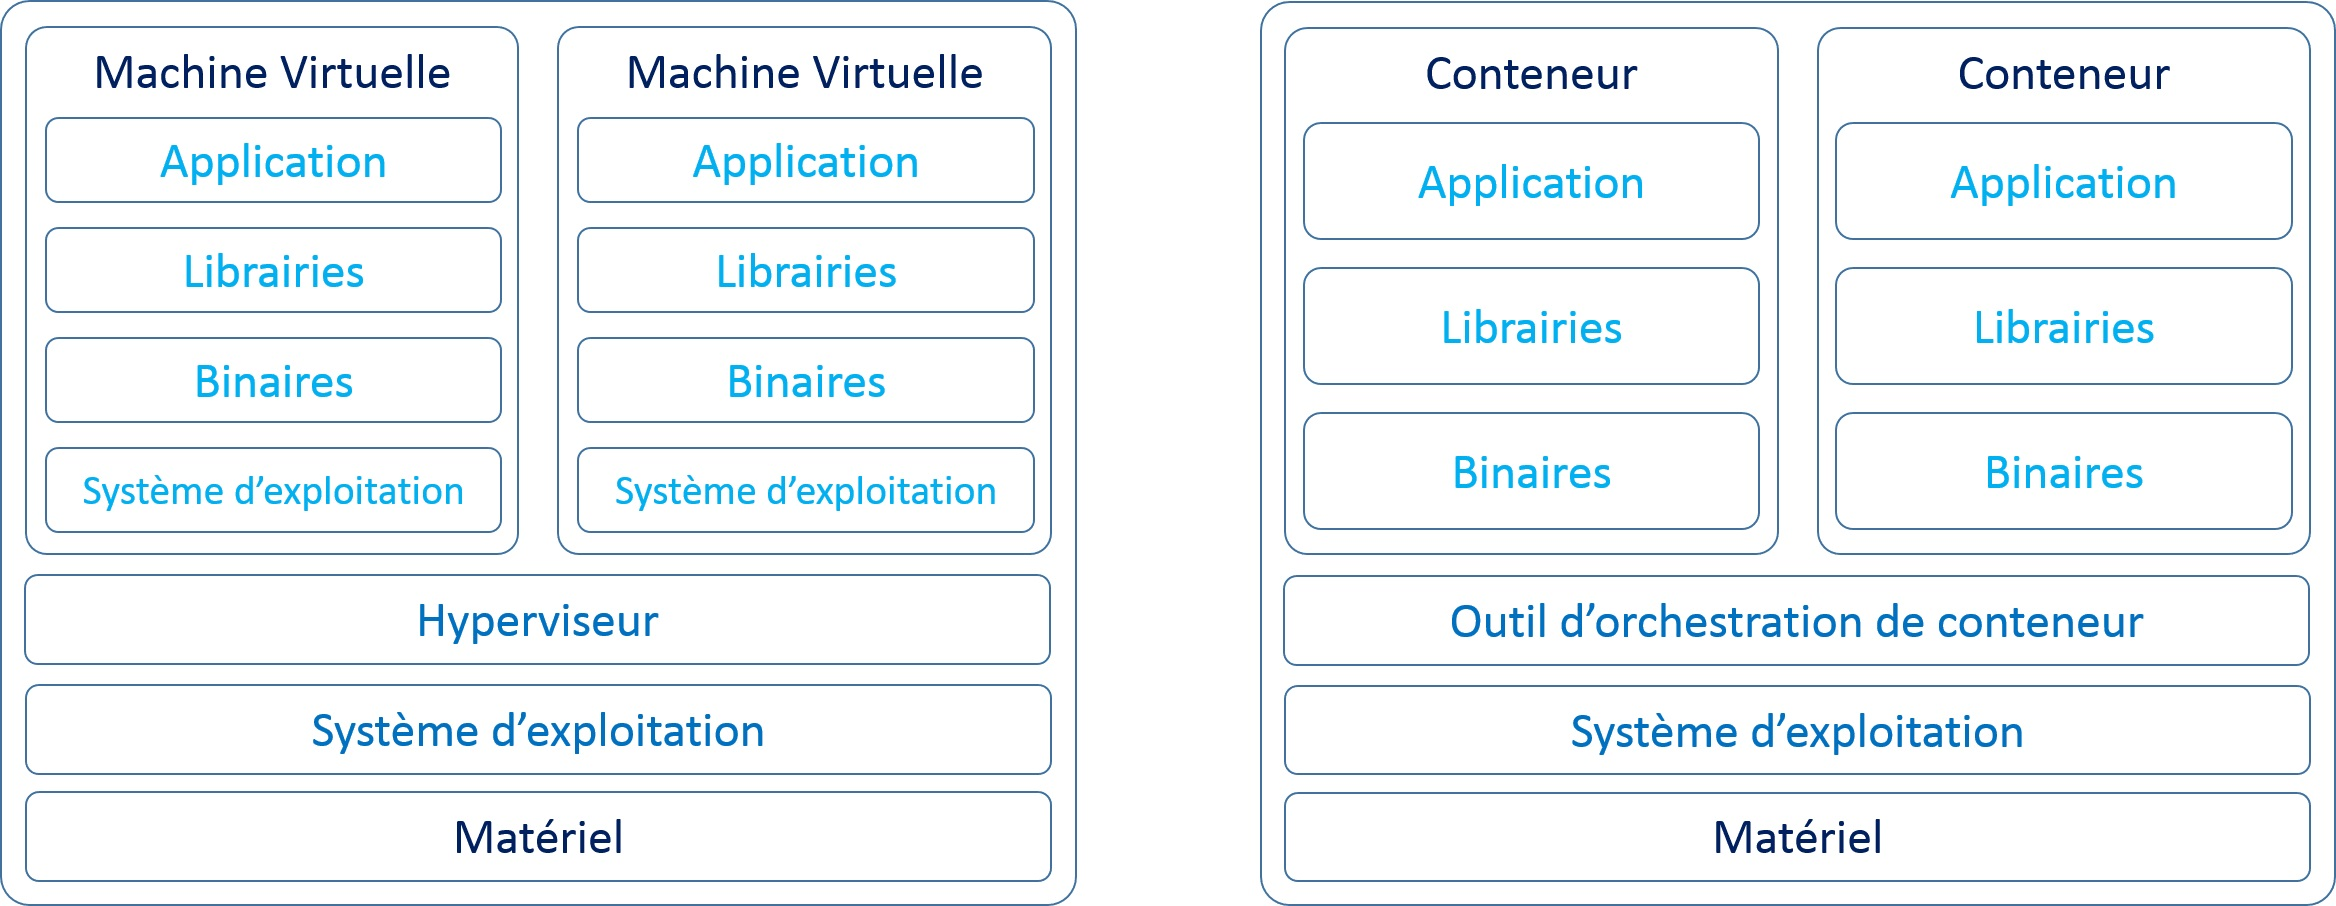
\includegraphics[scale=0.2]{vm-container.jpg}
\caption{Architecture de machine virtuelle (à gauche) ,et de conteneur (à droite) \cite{alibabacloud}}
\label{fig:vmvsconteneur}
\end{figure}
\subsection{Avantages et Inconvénients}
\subsubsection{Avantages de la virtualisation et de la migration}
La dynamicité de ce mécanisme de migration, confère une flexibilité dans la distribution et organisation des tâches de travail sur l'ensemble des ressources matérielles. Cela permet de répondre efficacement aux fluctuations des charges en mobilisant les conteneurs et machines virtuelles selon le besoin. Deux utilisations sont envisageables comme suit \cite{boutaba2013}.\par
D'une part, la migration permet de consolider les serveurs, en regroupant les instances virtuelles sur un nombre réduit de machines. Cette utilisation est particulièrement efficace dans le scénario de charge réduite et considérablement inférieure à la capacité de traitement totale disponible. Ceci afin de permettre la mise en veille ou la suspension des machines non exploitées et en l'occurrence réduire la consommation énergétique et ainsi les coûts engendrés.\par
D'une autre part, et dans les conditions opposées à celles susmentionnées, c'est à dire dans un environnement qui exige de grandes capacités de traitement, la précédente technique cause une surcharge sur les machines exploitées et par la suite une dégradation du temps de réponse et réduction du temps de disponibilité du service. Pour pallier ces contre-coups, la migration de machines virtuelles et de conteneurs est employée pour instaurer et assurer une uniformité dans la distribution des tâches entre les ressources physiques disponibles.\par
Ainsi, trouver un compromis optimal entre la consolidation de serveurs et l'équilibrage de charge est essentiel pour parvenir à une utilisation efficace des ressources dans les centres de données virtualisés.\par
Le mécanisme de migration permet aussi d'améliorer la localisation des données dans un réseau notamment dans des environnement Fog ou pour servir des applications hautement mobiles, résultant en une meilleure exploitation de la bande passante et la réduction du délai de communication.\par
De plus, ce mécanisme permet de conserver la continuité du service lors des maintenances routinières ou de pannes matérielles, et de minimiser les conséquences des erreurs humaines ou catastrophes naturelles en transférant les services critiques de façon réactive.
\subsubsection{Inconvénients}
Malgré ces avantages, la migration de VM (machine virtuelle) ou de container présentes quelques désavantages, parmi lesquels on cite:
\begin{itemize}
  \item Le coût en consommation de ressources engendré par l'opération de migration, en bande passante, temps de calcul CPU et disque.
  \item La discontinuité du service malgré l'existence de techniques qui réduisent ce dernier, mais qui reste toutefois inévitable.
  \item Dans le cloud public actuel, les machines virtuelles sont installées sur les mêmes machines physiques. Certaines des machines virtuelles travaillant dans le même sous-réseau ou serveur physique peuvent collaborer afin de satisfaire un service. La collaboration et les connexions entre VM via le réseau ainsi que le partage de ressources physiques augmentent le risque de vulnérabilité de sécurité, et de contamination par des VM malicieuses \cite{chandrakala2018}.
\end{itemize}
\subsection{Techniques de migration}
Nous nous intéresserons dans cette partie aux techniques de migration de conteneurs.\par
Nous distinguons deux type de migrations \cite{puliafito2019}:
\begin{itemize}
  \item La migration sans état: Le conteneur est redémarré de nouveau sur le nouvel hôte ce qui implique la perte de l'ancien état d'exécution. Elle se compose de deux étapes:
  \begin{enumerate}
    \item Lancement du nouveau conteneur sur la machine de destination.
    \item L'arrêt et suppression de l'ancien conteneur de la machine sources.
  \end{enumerate}
  \item La migration avec état: Dans ce type de migration, on conserve les données et contexte d'exécution lors du transfert, et trois techniques sont utilisées:
    \begin{enumerate}
      \item \emph{La migration à froid}: Le conteneur est arrêté, puis son état est sauvegardé afin d'être transféré vers le nœud de destination, où il reprendra son exécution. La durée de l'indisponibilité est égale à la durée totale de migration (voir figure \ref{fig:migration_a_froid}). Par contre, les pages mémoires ne sont transférées qu'une seule fois, ce qui réduit le temps de transfert et la quantité de données échangées.
      \begin{figure}[H]
      \centering
      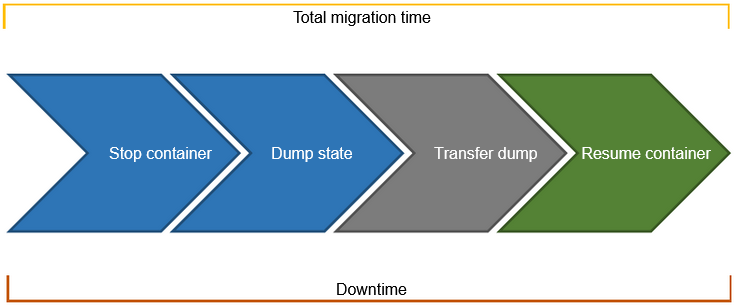
\includegraphics[scale=0.7]{migration_a_froid.png}
      \caption{La migration à froid}
      \label{fig:migration_a_froid}
      \end{figure}
      \item \emph{La migration à chaud}: Dans cette approche, une grande partie de l'état du conteneur est transférée en plein exécution. Il est ensuite suspendu seulement le temps du transfert d'une partie minimale de son état. Après quoi il reprend son exécution sur l'hôte de destination. On distingue trois sous catégories de migration à chaud:
        \begin{enumerate}
          \item La migration avec pré-copie.
          \item La migration avec post-copie.
          \item La migration hybride.
        \end{enumerate}
      \end{enumerate}
\end{itemize}
La migration avec pré-copie: La majorité de l'état du conteneur est transférée avant son arrêt. Puis, par itération, les pages mémoire altérées durant le transfert (dirty pages) sont envoyées. Le transfert se termine après un nombre prédéfini d'itérations. A ce moment-là seulement, le conteneur source interrompt son exécution et les dernières pages altérées sont transférées. Finalement, le nœud de destination reprend l'exécution (voir figure \ref{fig:migration_avec_precopie}).\par
\begin{figure}[H]
\centering
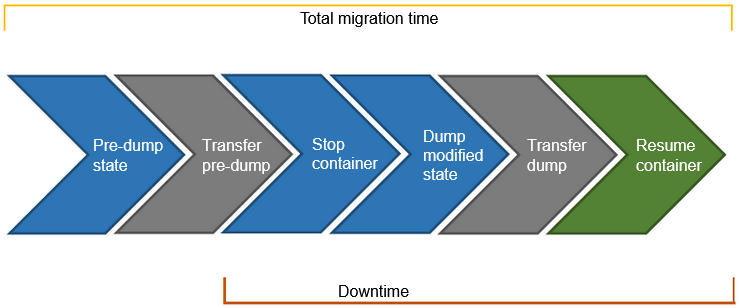
\includegraphics[scale=0.7]{migration_avec_precopie.png}
\caption{La migration avec pré-copie}
\label{fig:migration_avec_precopie}
\end{figure}
La migration avec post-copie: Par opposition à la technique précédente, le conteneur est d'abord suspendu et seulement le contexte d'exécution est transféré, et l'instance destination est lancée. Puis au besoin, la machine destination génère des demandes de pages défectueuses, auxquelles la machine source répond en envoyant ces pages (voir figure \ref{fig:migration_avec_postcopie}). C'est pour cette raison qu'elle est appelée migration fainéante.\par
\begin{figure}[H]
\centering
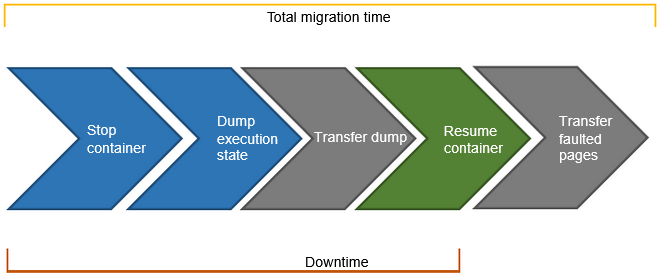
\includegraphics[scale=0.7]{migration_avec_postcopie.png}
\caption{La migration avec post-copie}
\label{fig:migration_avec_postcopie}
\end{figure}
La migration hybride: Les premières étapes coïncident avec celles de la migration avec pré-copie, à savoir la sauvegarde de l'état du conteneur en plein exécution et son transfert. Puis le conteneur source est arrêté, et une sauvegarde hybride est effectuée, une partie est transférée pour que le conteneur destination reprend son exécution (comme en pré-copie), et le reste des pages est transféré comme pages défectueuses à la demande (comme en post-copie) (voir figure \ref{fig:migration_hybride}).
\begin{figure}[H]
\centering
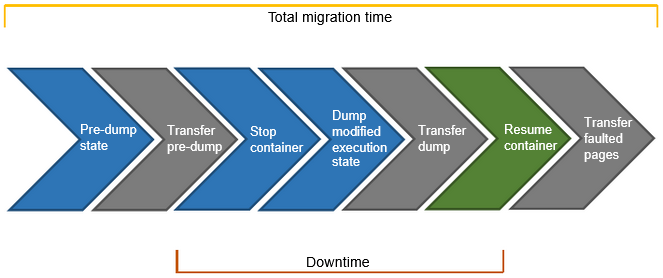
\includegraphics[scale=0.7]{migration_hybride.png}
\caption{La migration hybride}
\label{fig:migration_hybride}
\end{figure}

\subsection{Travaux et optimisation réalisés}
Les travaux réalisés dans le domaine de virtualisation et migration de ressources virtuels ont été classifiés selon la littérature en trois catégories selon l'objectif à optimiser \cite{rejiba2019}.
\begin{itemize}
  \item \emph{Optimisation du coût de la migration} : Visant soit à réduire les migrations coûteuses ou à trouver des compromis de coût de migration. Les processus de décision markovien constituent l'une des approches les plus utilisées pour modéliser le compromis de migration. Plus récemment, les efforts se sont progressivement déplacés vers la résolution du problème MDP en utilisant des approches apprentissage approfondies, qui ne nécessitent pas de connaissances préalables sur la dynamique de l'environnement MDP.
  \item \emph{Optimisation du temps de migration} : Les optimisations de migration focalisées sur l'axe du temps peuvent être divisées en optimisations proposées au niveau de la technologie de virtualisation et optimisations résultant de la prise d'actions proactives.
  \item \emph{Optimisation du taux d'erreur de la migration} : Les recherches sur ce sujet viennent exclusivement du domaine du cloud véhiculaire, à cause de la dynamicité le caractérisant, et qui peut potentiellement troubler le taux de succès de la migration. Ici, des techniques d'intelligence artificielle sont employées pour prédire la durée de disponibilité d'un véhicule dans une zone de couverture. Des protocoles de communication plus adaptés (comme le V2V) ont été aussi proposés.

\end{itemize}